Consider a solid domain with %constant mass density $\rho$ and
constant volume $\Omega \in \Rbb^3$, bounded by the surface $\partial \Omega$ within the time interval $t \in \tau=[0,T]$.
% Although the DGMPM has been developed within the finite strain framework, the equations considered here involve a configuration $\Omega$ that does not change during the deformation.
In that domain, a material particle is located in the Cartesian coordinates system by the vector $\vect{x}=x_\alpha \vect{e}_\alpha$, following the convention of implicit summation over repeated indices.

\subsection{The model equation}
We focus here on the transport of an arbitrary scalar quantity $q$ in that domain, governed by the advection equation:
\begin{equation}
  \label{eq:advection_equation}
  \drond{q}{t}(\vect{x},t) +  \nablav \cdot \vect{F}(\vect{x},t) = 0 \quad \forall \:\vect{x},t \in \Omega \times \tau
\end{equation}
where $\nablav \cdot (\bullet)$ is the right divergence operator, and $\vect{F}=q(\vect{x},t)s_\alpha \vect{e}_\alpha$, the flux vector.
In the expression of the flux vector, $s_\alpha \in \Rbb$ is the speed at which the quantity $q$ is advected in direction $\vect{e}_\alpha$.
For the linear advection equation considered here, these celerities are constant and equation \eqref{eq:advection_equation} can be rewritten as:
\begin{equation}
  \label{eq:advection_equation_sum}
  \drond{q}{t}(\vect{x},t) +  s_\alpha \drond{q}{x_\alpha}(\vect{x},t) = 0\quad \forall \:\vect{x},t \in \Omega \times \tau
\end{equation}

\subsection{DGMPM space discretization}
The continuum body $\Omega$ is discretized into a set of $N_p$ material points in a Cartesian grid made of $N_n$ nodes and $E$ non-overlapping cells of volume $\Omega^e$.
The boundary of the computational domain is defined by the set of faces separating empty cells from those containing particles (see figure \ref{fig:domain} for a two-dimensional example).
\begin{figure}[ht]
  \centering
  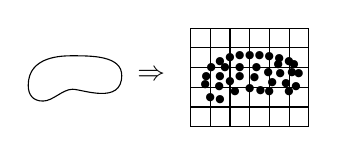
\begin{tikzpicture}[scale=0.25]
  % \draw[step=1.0,black,thin] (-3.,-1.) grid (3,4.);
  % \draw (-3,-1) -- (3,-1) -- (3,4) -- (-3,4) -- (-3,-1);
  \begin{scope}[scale=0.5]
    \draw (-3,0.6) .. controls +(1,0) and +(-1,0) .. (0,1.8)  
    .. controls +(1,0) and +(0,-3) .. (5,3.2) 
    .. controls +(0,2) and +(2,0)  .. (0,5.2) 
    .. controls +(-1,0) and +(0,3) .. (-4.5,2.2) 
    .. controls +(0,-1) and +(-1,0).. (-3,0.6) ;
    \begin{scope}  % pour limiter la portée du clip
      \clip (-3,0.6) .. controls +(1,0) and +(-1,0) .. (0,1.8) 
      .. controls +(1,0) and +(0,-3) .. (5,3.2)
      .. controls +(0,2) and +(2,0)  .. (0,5.2)
      .. controls +(-1,0) and +(0,3) .. (-4.5,2.2)
      .. controls +(0,-1) and +(-1,0).. (-3,0.6);
    \end{scope}
    %\node[below] at (0,1) {$\Omega$};
  \end{scope}
  \node at (4.,1.62) {$\Rightarrow$};
  \begin{scope}[shift={(9,0)}]
    \draw[step=1.0,black,thin] (-3.,-1.) grid (3,4.);
    % contour
    \node at (0,0.9) {\scriptsize$\bullet$}  ;
    \node at (2.5,1.65) {\scriptsize$\bullet$}  ; 
    \node at (0,2.6) {\scriptsize$\bullet$}  ;
    \node at (-2.25,1.1) {\scriptsize$\bullet$}  ; 
    \node at (-1.5,0.35) {\scriptsize$\bullet$}  ; 
    \node at (-2.,0.45) {\scriptsize$\bullet$} ;
    \node at (-2.2,1.5) {\scriptsize$\bullet$}  ; 
    \node at (-1.5,2.3) {\scriptsize$\bullet$} ; 
    \node at (2.35,1.) {\scriptsize$\bullet$}  ;
    \node at (2.25,2.15) {\scriptsize$\bullet$}  ;
    \node at (0.55,0.8) {\scriptsize$\bullet$}  ; 
    \node at (-0.5,2.6) {\scriptsize$\bullet$};
    \node at (0.5,2.59) {\scriptsize$\bullet$}  ;
    \node at (1.5,2.45) {\scriptsize$\bullet$}  ;
    \node at (1,0.75) {\scriptsize$\bullet$}; 
    \node at (2,0.75) {\scriptsize$\bullet$}  ;
    \node at (2,2.3) {\scriptsize$\bullet$}  ;
    \node at (1,2.55) {\scriptsize$\bullet$}  ;
    \node at (-1,2.5) {\scriptsize$\bullet$}  ; 
    \node at (-1.95,2.) {\scriptsize$\bullet$}  ;
    % interior
    \node at (-1.5,1.5) {\scriptsize$\bullet$}  ; 
    \node at (-1.25,2.) {\scriptsize$\bullet$}  ;
    \node at (-0.75,0.75) {\scriptsize$\bullet$}  ; 
    \node at (-1.55,1.){\scriptsize$\bullet$} ;
    \node at (-0.5,1.5) {\scriptsize$\bullet$}  ; 
    \node at (-0.5,2.) {\scriptsize$\bullet$}  ;
    \node at (0.25,1.45) {\scriptsize$\bullet$}  ;
    \node at (0.35,2.) {\scriptsize$\bullet$}  ;
    \node at (0.95,1.75) {\scriptsize$\bullet$}  ;
    \node at (1.15,1.2) {\scriptsize$\bullet$} ;
    \node at (1.45,2.15) {\scriptsize$\bullet$}  ; 
    \node at (1.55,1.65) {\scriptsize$\bullet$}  ;
    \node at (1.85,1.15) {\scriptsize$\bullet$}  ; 
    \node at (2.15,1.75) {\scriptsize$\bullet$}  ;
    \node at (-1.,1.25) {\scriptsize$\bullet$}  ;
    % \draw(3,0.5) -- (3.4,0.5) node [right]  {$\Omega_g$};
  \end{scope}
\end{tikzpicture}

%%% Local Variables:
%%% mode: latex
%%% TeX-master: "../presentation"
%%% End:

  \caption{Representation of a continuum body by a set of material points in a regular grid in $\Rbb^2$.}
  \label{fig:domain}	
\end{figure}
%%%%%
Even though MPM, and in turn DGMPM, have been developed for solid dynamics based on the balance equation of linear momentum, the formulation can be extended to equation \eqref{eq:advection_equation} by means of a fictitious mass density $\rho$.
Indeed, the methods rely on the representation of the mass density that weights the time partial derivative of the hyperbolic equation by means of a delta Dirac characteristic function:
%%%%
%MPM and DGMPM formulations for solid dynamics are based on representation of the mass density arising in the linear momentum balance equation by means of a delta Dirac characteristic function.
%%%%
% In that computational grid, the mass density is described based on the delta Dirac characteristic function and particles masses:
\begin{equation}
  \label{eq:mass_density_DGMPM}
  \rho\(\vect{x}\) =  \sum_{I=1}^{N_p} m_I \delta\(\vect{x}^I - \vect{x}\)
\end{equation}
where $\vect{x}^I$ is the position of the $I$th material point and $m_I$ the associated mass.
In the following, a unit mass density is assumed to derive the DGMPM.
% Even though equations \eqref{eq:advection_equation} and \eqref{eq:advection_equation_sum} do not involve the mass density, the approximation \eqref{eq:mass_density_DGMPM} is used hereinafter with a unit mass density.
Analogously to FEM and MPM, the quantity $q$ is approximated on the background grid as:
\begin{equation}
  \label{eq:DGMPM_node2points}
  q(\vect{x},t) = \sum^{N_n}_{i=1} S_{i}(\vect{x})q^i(t) 
\end{equation}
with $q^i$ the quantity at node $i$ and $S_{i}(\vect{x})$ the shape function attached to that node.
Note that the convention of denoting particle and nodal fields by uppercase and lowercase indices respectively is used in the remainder of the paper.

The key idea of DG methods is to allow jump of fields across mesh elements faces by using broken polynomial spaces for the approximate solution \cite{DiPietro}:
\begin{equation}
\Vscr^k = \{ \Vc \in H^k(\Omega^e) \} \quad ;\quad \Vscr_h^k = \{\Vc \in \Pscr^k(\Omega^e) \} \subset \Vscr^k
\end{equation}
$H^k(\Omega^e)$ being the Sobolev space, and $\Pscr^k(\Omega^e)$ the space of polynomials of degree $k$ in $\Omega^e$.
We restrict our attention here to linear polynomials ($k=1$).
Multiplying equation \eqref{eq:advection_equation} by a test function $\Vc$ yields the element-wise weak formulation of the problem:
\begin{equation}
  \label{eq:weak_form}
  \begin{aligned}
    &\textit{Find $q \in \Vscr_h^1$ such that }\forall e \\
    &\int_{\Omega^e} \Vc \drond{q}{t} \: d\Omega + \int_{\Omega^e}  \Vc \:  \nablav \cdot \vect{F}  \: d\Omega    = 0 \quad \forall \: \Vc,t \in  \Vscr_h^1\times \tau
  \end{aligned}
\end{equation}
Then, the use of Gauss' divergence theorem leads to:
\begin{equation}
  \label{eq:DGMPM_weak_form}
  \begin{aligned}
    &\textit{Find $q \in \Vscr_h^1$ such that }\forall e \\
    &\int_{\Omega^e} \[\drond{q}{t} \Vc - \vect{F} \cdot \nablav \Vc \] d\Omega   + \int_{\partial \Omega^e} \(\vect{F}\cdot \vect{n}\)  \Vc \: d\Gamma = 0 \quad \forall \: \Vc,t \in  \Vscr_h^1\times \tau
  \end{aligned}
\end{equation}
where $\partial \Omega^e$ is the boundary of the $e$th element with outward normal vector $\vect{n}$, and $\nablav(\bullet)$ is the gradient operator.
%The dot operator $\Fcb\cdot \vect{N}$ denotes the inner product between the outward normal vector and every component of the flux, thus yielding the intercell flux, written $\Fcb_N$ for simplicity.
The inner product $\vect{F}\cdot \vect{n}$, corresponding to intercell flux, is written $F_n$ for simplicity.
Next, the introduction of specific fields:
\begin{equation}
  \label{eq:specific_quantities}
  q = \rho \bar{q} \quad ; \quad \vect{F} = \rho \bar{\vect{F}} =\rho \vect{s} \bar{q}
\end{equation}
combined with the definition of mass density \eqref{eq:mass_density_DGMPM}, leads to the following weak form:
\begin{equation} 
  \label{eq:DGMPM_discrete_weak}
  \sum_{I=1}^{N_p} m_I\[\drond{\bar{q}}{t}  \Vc - \vect{s}\bar{q} \cdot \nablav \Vc \]_{|\vect{x}=\vect{x}^I} + \int_{\partial \Omega^e} F_n  \Vc \: d\Gamma = 0 \quad \forall \: \Vc,t \in  \Vscr_h^1\times \tau
\end{equation}
Introduction of the DGMPM approximation \eqref{eq:DGMPM_node2points} and arbitrariness of the test field in the weak form \eqref{eq:DGMPM_discrete_weak} finally provide the semi-discrete system that must be solved on the grid:
\begin{equation}
  \label{eq:DGMPM_semi_discrete}
  \sum_{I=1}^{N_p}\[ S_{iI} m_I S_{jI} \drond{\bar{q}^j}{t}  - \drond{S_{iI}}{x_\alpha} m_I S_{jI} s_\alpha \bar{q}^j\] + \int_{\Gamma_e} S_i(\vect{x}) F_n  \: d\Gamma =  0  \quad \forall \: t \in  \tau
\end{equation}
or, in matrix form:
\begin{equation}
  \label{eq:DGMPM_semi_discrete_matrix}
  M_{ij} \drond{\bar{q}^j}{t} - K^\alpha_{ij} s_\alpha \bar{q}^j + \hat{F}^i = 0  
\end{equation}
%The particles play the role of integration points in volume integrals owing to the delta Dirac characteristic function.
%Hence, as for MPM, the consistent mass matrix $M_{ij}$ may be singular due to reduced integration, so that the diagonally lumped mass matrix $M^L_i=\sum_{j=1}^{N_n} M_{ij}$ is used \cite{Love}.
\review{
  \begin{remark}
    As for MPM, the particle-based quadrature rule yields a consistent mass matrix $M_{ij}$ that may be singular due to reduced integration.
    This can be circumvented by resorting to the diagonally lumped mass matrix $M^L_i=\sum_{j=1}^{N_n} M_{ij}$ is used \cite{Love}.
    The aforementioned numerical trick, which is also employed in explicit FEM \cite{Belytschko} for efficiency purposes, can be avoided within the MPM owing to recent works.
    Indeed, the use of \textit{moving least squares} \cite{IMPM} or \textit{spline interpolation} \cite{MPM_BSpline1,MPM_BSpline2} techniques enables the evaluation of a reconstructed function ot Gauss point locations. 
    In these versions of the MPM, the particles are no longer seen as integration points. %so that higher-order approximations are possible regardless of the distribution of material points.
    Similar reconstructions can be considered within the DGMPM, which would amount to provide an arbitrary background grid to a DG scheme.
    This is, however, out of the scope of the present work.
  \end{remark}
  \begin{remark}
    The DGMPM discretization can be constructed upon regular grids that allow the straightforward building of an orthonormal approximation basis.
    In that case, the mass matrix is naturally diagonal provided the derivation of a modal formulation as can be done for DGFEM \cite{Hesthaven}.  
  \end{remark}
}

The DGMPM discrete system is finally derived by dividing the time interval $\tau$ into $N_t$ subintervals and using the explicit forward Euler method:
\begin{equation}
  \label{eq:DGMPM_discrete}
  M^L_i \frac{\bar{q}^{i,k+1} - \bar{q}^{i,k}}{\Delta t^{k} } = K^\alpha_{ij} s_\alpha\bar{q}^{j,k} - \hat{F}^{i,k}  
\end{equation}
where the superscripts $(\bullet)^{i,k}$ denote a field evaluated at node $i$ and time step $k$.
Alternatively, a second-order Runge-Kutta (RK2) explicit time discretization may be employed, leading to the following two-stage discrete form:
\begin{equation}
  \label{eq:DGMPM_discrete_RK2}
  \begin{aligned}
    & M^L_i \frac{\bar{q}^{i,k+1/2} - \bar{q}^{i,k}}{\Delta t^{k} } = \frac{1}{2}\(K^\alpha_{ij} s_\alpha\bar{q}^{j,k} - \hat{F}^{i,k}\)  \\
    & M^L_i \frac{\bar{q}^{i,k+1} - \bar{q}^{i,k}}{\Delta t^{k} } = K^\alpha_{ij} s_{\alpha}\bar{q}^{j,k+1/2} - \hat{F}^{i,k+1/2}
  \end{aligned}
\end{equation}

\subsection{Computation of intercell fluxes}
The relaxation of the continuity of fields across cells interfaces introduced by the DG approximation allows to define Riemann problems at element faces in the direction $x_n=\vect{x}\cdot{n}$:
\begin{equation}
  \label{eq:RP_mesh}
  \begin{aligned}
    &\drond{q}{t} + \drond{F_n}{x_n} = 0  \\
    & q(x_n,0)= \left\lbrace 
      \begin{aligned}
        & q^{-} \text{ if } x_n <0 \\
        & q^{+} \text{ if } x_n > 0
      \end{aligned}
        \right.
  \end{aligned}
\end{equation}
where the $q^{\pm}$ are downwind and upwind states.
The use of DG approximation can be seen as a duplication of nodes so that those states can be obtained by averaging nodal fields on each side of the interface as depicted in figure \ref{fig:2D_edge} for a two-dimensional case.
By doing so, only one Riemann problem per interface rather than nodal ones is considered, thus avoiding a dramatic increase in computational time.
%\review{Nevertheless, nodal Riemann problems might be considered for an extension of the method to higher-order approximations.}
\begin{figure}[h!]
  \centering
  \begin{tikzpicture}[scale=0.5]
  \draw (10.,0.) -- (12.,6.) ; 
  \draw[fill=black] (9.85,0.1) circle (0.1) node [left] {$1$};	
  \draw[fill=black] (10.2,-0.0) circle (0.1) node [right] {$2$};	
  \draw[fill=black] (11.85,6.1) circle (0.1) node [left] {$4$};	
  \draw[fill=black] (12.2,6) circle (0.1) node [right] {$3$};	
  \draw[->,very thick] (11.,3.) -- (12,3 -1/3) node [right,below] {$X_N$}; 
  \node at (8,3.5) {$\vect{\Qc}_{L} = \frac{\vect{\Qc}_1 + \vect{\Qc}_4}{2}$}; \node at (14.5,3.5) {$\vect{\Qc}_{R} = \frac{\vect{\Qc}_2 + \vect{\Qc}_3}{2}$};
\end{tikzpicture}

  \caption{Duplication of nodes at an interface and building of initial conditions of the Riemann problem (2D).}
  \label{fig:2D_edge}
\end{figure}
As for the original formulation of the DGMPM \cite{DGMPM}, the numerical flux at a given interface is based on the stationary solution $q^*$ of the Riemann problem \eqref{eq:RP_mesh} according to Godunov's method \cite{Godunov_method}.
For the linear advection, the stationary solution is simply that of the upwind side, namely:
\begin{equation}
  \label{eq:stationary_state}
  \left\lbrace
    \begin{aligned}
      & q^* = q^{-} \quad \text{if $s_n>0$}\\
      & q^* = q^{+} \quad \text{if $s_n<0$}
    \end{aligned}
    \right.
\end{equation}
where $s_n=\vect{s}\cdot\vect{n}$, so that the intercell flux at a given interface reads $F_n=s_n q^*$.

% \subsubsection{Transverse corrections}
The method derived above for the computation of normal fluxes can be seen as the Donor-Cell Upwind method (DCU) \cite{Leveque} in which only the influence of upwind neighbor cells is considered.
For multi-dimensional problems, however, waves can travel in several directions so that contributions coming from corner cells must be taken into account in order to improve accuracy and stability of the numerical scheme.
The Corner Transport Upwind method (CTU) \cite{Colella_CTU} consists in considering contributions propagating in bias and coming from upwind cells sharing only a node (in two dimensions) with another.
This approach has been developed for finite volumes in which fields are cell-wise constant and allows to improve the Courant condition.
The approach is now reformulated for DGMPM, based on edge-wise constant fields within Riemann problems.

At each cell interface, one defines left-going and right-going fluctuations as:
\begin{equation}
  \label{eq:fluctuations}
  \Ac^-(\Delta q) = F_n(q^*) - F_n(q^-) \quad ;  \quad \Ac^+(\Delta q) = F_n(q^+)-F_n(q^*) 
\end{equation}
From equation \eqref{eq:fluctuations} and the definition of the stationary state $q^*$ \eqref{eq:stationary_state}, one of the fluctuation obviously vanishes for the scalar linear advection equation.
The non-zero fluctuation, on the other hand, characterizes a wave that carries a jump discontinuity $\Delta q$ at speed $s_n$ in the direction $\vect{n}$.
This jump influences the state vector $q$ in the neighbor cell so that the the initial data in the Riemann problems formulated on adjacent edges are changed.
To illustrate the above discussion, let's consider the patch of two-dimensional regular grid cells of length $\Delta x$ shown in figure \ref{fig:ctu_perso}.
\begin{figure}[ht]
  \centering
  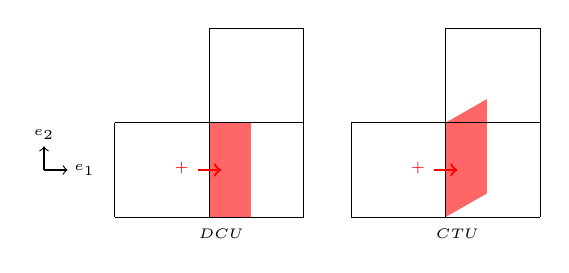
\begin{tikzpicture}[scale=0.6]
  \fill[Red!60] (0,0) rectangle (.875,-2);
  \draw (-2,0) -- (2,0.);\draw (0.,2) -- (0,-2.);\draw (0,2) -- (2,2);
  \draw (-2.,-2.) -- (2.,-2.);\draw (2,2.) -- (2,-2.);\draw (-2,-2) -- (-2,0);
  \begin{tiny}
    \draw[->,thick,Red] (-.25,-1.) node [left] {$\Ac^+$} -- (.25,-1.) ;
    \draw[->] (-3.5,-1.) -- (-3,-1.) node[right] {$\vect{e}_1$};
    \draw[->] (-3.5,-1.) -- (-3.5,-0.5) node[above] {$\vect{e}_2$};
    \node at (0.25,-2.35) {$DCU$};
  \end{tiny}
  \begin{scope}[shift={(5.,0.)}]
    \fill[Red!60] (0,0) rectangle (.875,-2);
    \fill[Red!60] (0,0) -- (.875,0) -- (.875,.5) -- (0.,0.); %% Red triangle
    \fill[white] (0,0-2) -- (.875,0-2) -- (.875,.5-2) -- (0.,0.-2); %% White triangle
    \draw (-2,0) -- (2,0.);\draw (0.,2) -- (0,-2.);\draw (0,2) -- (2,2);
    \draw (-2.,-2.) -- (2.,-2.);\draw (2,2.) -- (2,-2.);\draw (-2,-2) -- (-2,0);
    \begin{tiny}
      \draw[->,thick,Red] (-.25,-1.) node [left] {$\Ac^+$} -- (.25,-1.) ;
      \node at (0.25,-2.35) {$CTU$};
    \end{tiny}    
  \end{scope}
\end{tikzpicture}

%%% Local Variables:
%%% mode: latex
%%% TeX-master: "../../presentation"
%%% End:

  \caption{Illustration of the influence of fluctuations on fluxes computed at adjacent cells interfaces.}
  \label{fig:ctu_perso}
\end{figure}
% Since the choice is made in DGMPM to consider constant states $q$ on each side of an interface in order to solve only one Riemann problem per edge,
Assuming that the speed vector $\vect{s}$ is such that $s_1,s_2>0$, the solution of the Riemann problem on edge $(i)$ yields the fluctuation $\Ac^+(\Delta q^{(i)})$ which travels the distance $s_1\Delta t$ in cell C.
On the other hand, the flux through edge $(j)$ reads \cite{Toro}:
\begin{equation}
  \label{eq:flux_Toro}
  F_n^{(j)}=\frac{1}{\Delta t}\int_{0}^{\Delta t} s_2 \tilde{q} dt
\end{equation}
where $\tilde{q}$ is the upwind state at edge $(j)$.
When using DCU, this constant state is built from nodal values in cell $C$ and is written $q^{-,(j)}$.
Alternatively, $\tilde{q}$ is taken in CTU as the average of states $q^{-,(i)}$ and $q^{-,(j)}$, weighted by the portion of edge $(j)$ along which they respectively act at time $t$, namely:
\begin{equation}
  \label{eq:mean_q}
  \tilde{q} = \frac{s_1 t \:q^{-,(i)} + (\Delta x - s_1t \:)q^{-,(j)} }{\Delta x}
\end{equation}
Thus, integral \eqref{eq:flux_Toro} yields:
\begin{equation}
  F_n^{(j)}=s_2 \frac{s_1 \Delta t}{\Delta x}q^{-,(i)}  + s_2\frac{\Delta x -s_1 \Delta t}{\Delta x} q^{-,(j)}
\end{equation}
which can be rewritten:
\begin{equation}
  \label{eq:corrected_flux}
  F_n^{(j)}=s_2q^{-,(j)} -  \frac{1}{2}\frac{\Delta t}{\Delta x}s_2s_1(q^{-,(j)}  - q^{-,(i)}) = F_n^{(j)}(q^{-,(j)}) - \frac{1}{2}\frac{\Delta t}{\Delta x}\Bc^+ \Ac^+(\Delta q^{(i)})
\end{equation}
where $F_n^{(j)}(q^{-,(i)})$ is the flux through the edge $(j)$ resulting from the DCU, and $\Bc^+ \Ac^+(\Delta q^{(i)})$ is a transverse correction coming from edge $(i)$.
It then comes out that the CTU leads to the same corrections in DGMPM than it does in FVM \cite{Leveque}.

\subsection{Solution scheme}
Suppose that the quantity $q$ is known at every material points that discretize a solid domain $\Omega$ at a time increment $t^k $.
Since the volume is assumed constant, the lumped mass and pseudo-stiffness matrices $M_{i}^L$ and $K_{ij}^\alpha$ can be computed once and for all at the beginning of the computation.
Then, the DGMPM procedure followed to update the field between $t^k$ and $t^{k+1}$ consists in the following steps:
\begin{itemize}
\item[(a)] project the field onto the grid by solving for the $\bar{q}^i$ the conservation of volume quantities \cite{DGMPM}:
  \begin{equation}
    \label{eq:DGMPM_points2nodes}
    M^L_i \bar{q}^i = \sum_{I=1}^{N_p} S_{iI} m_I \bar{q}^I 
  \end{equation}
\item[(b)] compute intercell fluxes by using either DCU or CTU approach, as well as volume fluxes.
\item[(c)] advance the solution in time by solving the discrete system \eqref{eq:DGMPM_discrete} or \eqref{eq:DGMPM_discrete_RK2}
\item[(d)] interpolate the updated fields $\bar{q}^i$ to material points according to equation \eqref{eq:DGMPM_node2points}
\end{itemize}

%%% Local Variables:
%%% mode: latex
%%% TeX-master: "manuscript"
%%% End:
